% Options for packages loaded elsewhere
\PassOptionsToPackage{unicode}{hyperref}
\PassOptionsToPackage{hyphens}{url}
%
\documentclass[
]{article}
\usepackage{amsmath,amssymb}
\usepackage{lmodern}
\usepackage{iftex}
\ifPDFTeX
  \usepackage[T1]{fontenc}
  \usepackage[utf8]{inputenc}
  \usepackage{textcomp} % provide euro and other symbols
\else % if luatex or xetex
  \usepackage{unicode-math}
  \defaultfontfeatures{Scale=MatchLowercase}
  \defaultfontfeatures[\rmfamily]{Ligatures=TeX,Scale=1}
\fi
% Use upquote if available, for straight quotes in verbatim environments
\IfFileExists{upquote.sty}{\usepackage{upquote}}{}
\IfFileExists{microtype.sty}{% use microtype if available
  \usepackage[]{microtype}
  \UseMicrotypeSet[protrusion]{basicmath} % disable protrusion for tt fonts
}{}
\makeatletter
\@ifundefined{KOMAClassName}{% if non-KOMA class
  \IfFileExists{parskip.sty}{%
    \usepackage{parskip}
  }{% else
    \setlength{\parindent}{0pt}
    \setlength{\parskip}{6pt plus 2pt minus 1pt}}
}{% if KOMA class
  \KOMAoptions{parskip=half}}
\makeatother
\usepackage{xcolor}
\usepackage[margin=1in]{geometry}
\usepackage{graphicx}
\makeatletter
\def\maxwidth{\ifdim\Gin@nat@width>\linewidth\linewidth\else\Gin@nat@width\fi}
\def\maxheight{\ifdim\Gin@nat@height>\textheight\textheight\else\Gin@nat@height\fi}
\makeatother
% Scale images if necessary, so that they will not overflow the page
% margins by default, and it is still possible to overwrite the defaults
% using explicit options in \includegraphics[width, height, ...]{}
\setkeys{Gin}{width=\maxwidth,height=\maxheight,keepaspectratio}
% Set default figure placement to htbp
\makeatletter
\def\fps@figure{htbp}
\makeatother
\setlength{\emergencystretch}{3em} % prevent overfull lines
\providecommand{\tightlist}{%
  \setlength{\itemsep}{0pt}\setlength{\parskip}{0pt}}
\setcounter{secnumdepth}{-\maxdimen} % remove section numbering
\usepackage{pdflscape}
\newcommand{\blandscape}{\begin{landscape}}
\newcommand{\elandscape}{\end{landscape}}
\ifLuaTeX
  \usepackage{selnolig}  % disable illegal ligatures
\fi
\IfFileExists{bookmark.sty}{\usepackage{bookmark}}{\usepackage{hyperref}}
\IfFileExists{xurl.sty}{\usepackage{xurl}}{} % add URL line breaks if available
\urlstyle{same} % disable monospaced font for URLs
\hypersetup{
  pdftitle={Supplementary Figures},
  hidelinks,
  pdfcreator={LaTeX via pandoc}}

\title{\textbf{Supplementary Figures}}
\author{}
\date{\vspace{-2.5em}}

\begin{document}
\maketitle

\hypertarget{navigating-sustainability-and-health-trade-offs-in-global-seafood-systems}{%
\section{Navigating sustainability and health trade-offs in global
seafood
systems}\label{navigating-sustainability-and-health-trade-offs-in-global-seafood-systems}}

Authors: James PW Robinson, Angus Garrett, Juan Carlos Paredes Esclapez,
Eva Maire, Robert WR Parker, Christina C Hicks, Nicholas AJ Graham

\newpage

\begin{center}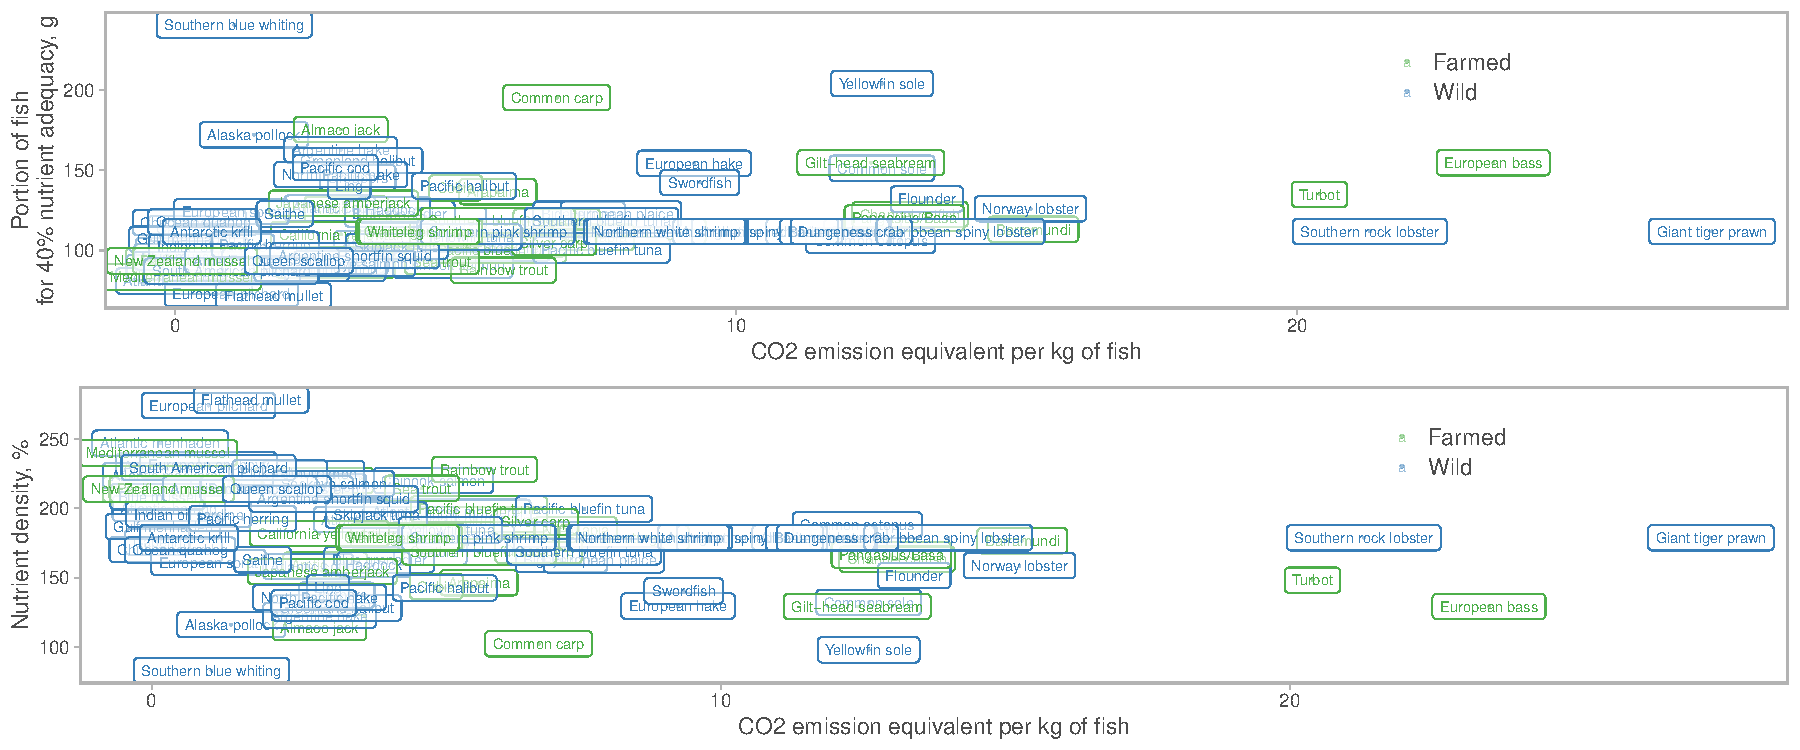
\includegraphics[height=0.8\textheight]{fig/final/FigureS1_nutrient_ghg} \end{center}

\textbf{Fig. S1. Nutritional value and carbon footprint of seafood
species} Points are kg CO2-eq of each species and its corresponding the
nutrient density (\%). Nutrient density is the summed contribution of a
100g portion to recommended intakes of five nutrients (calcium, iron,
selenium, zinc, omega-3 fatty acids) (recommended daily intakes for
adults (18-65 years old)).

\newpage

\begin{center}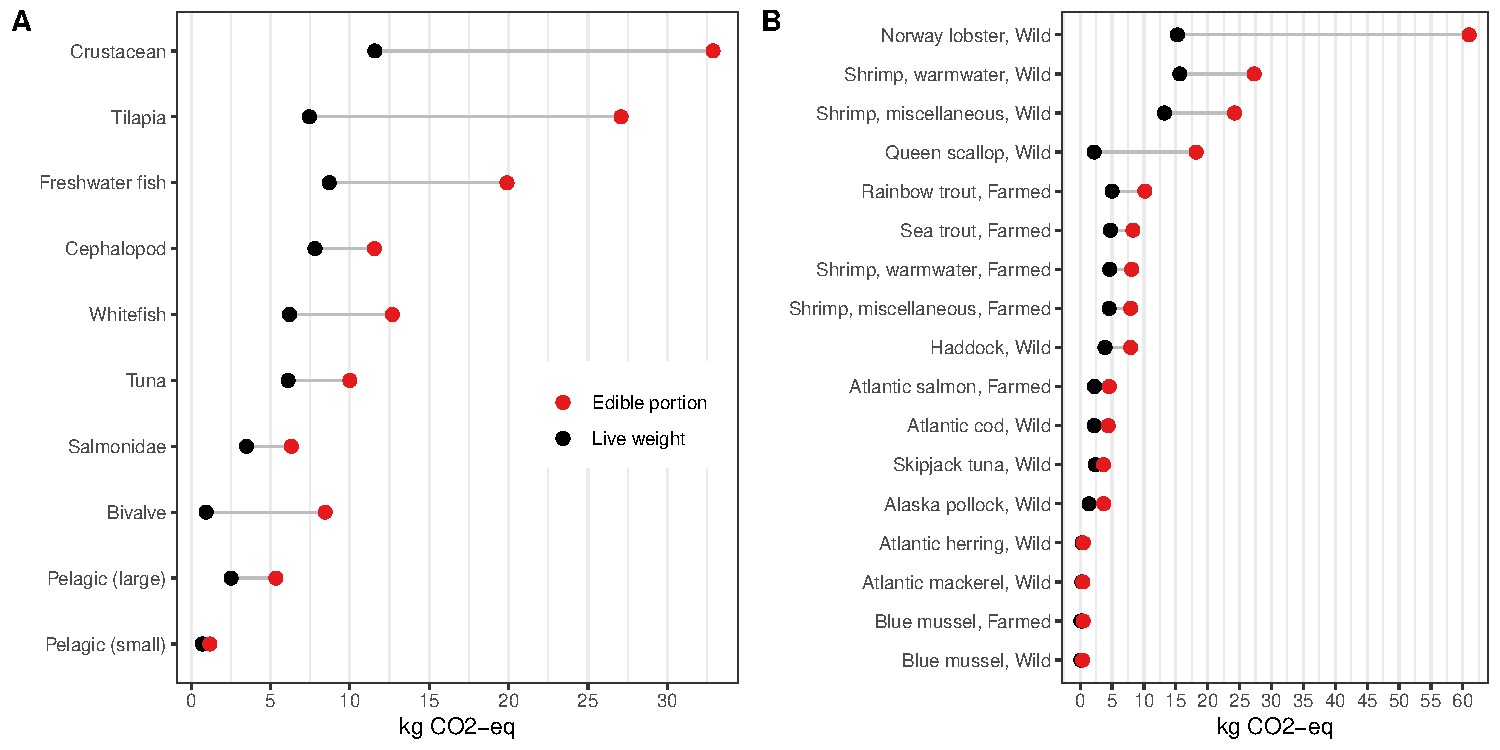
\includegraphics[height=0.8\textheight]{fig/final/Figure_SX_GHG_edible} \end{center}

\textbf{Fig. S2. Carbon footprint of seafood species corrected for
edible portions} Points are kg CO2-eq for groups of global seafood
products (A) and UK-specific seafood productions (B), showing
unprocessed estimates (black) and estimates for processed, edible
seafood (red).

\newpage

\begin{center}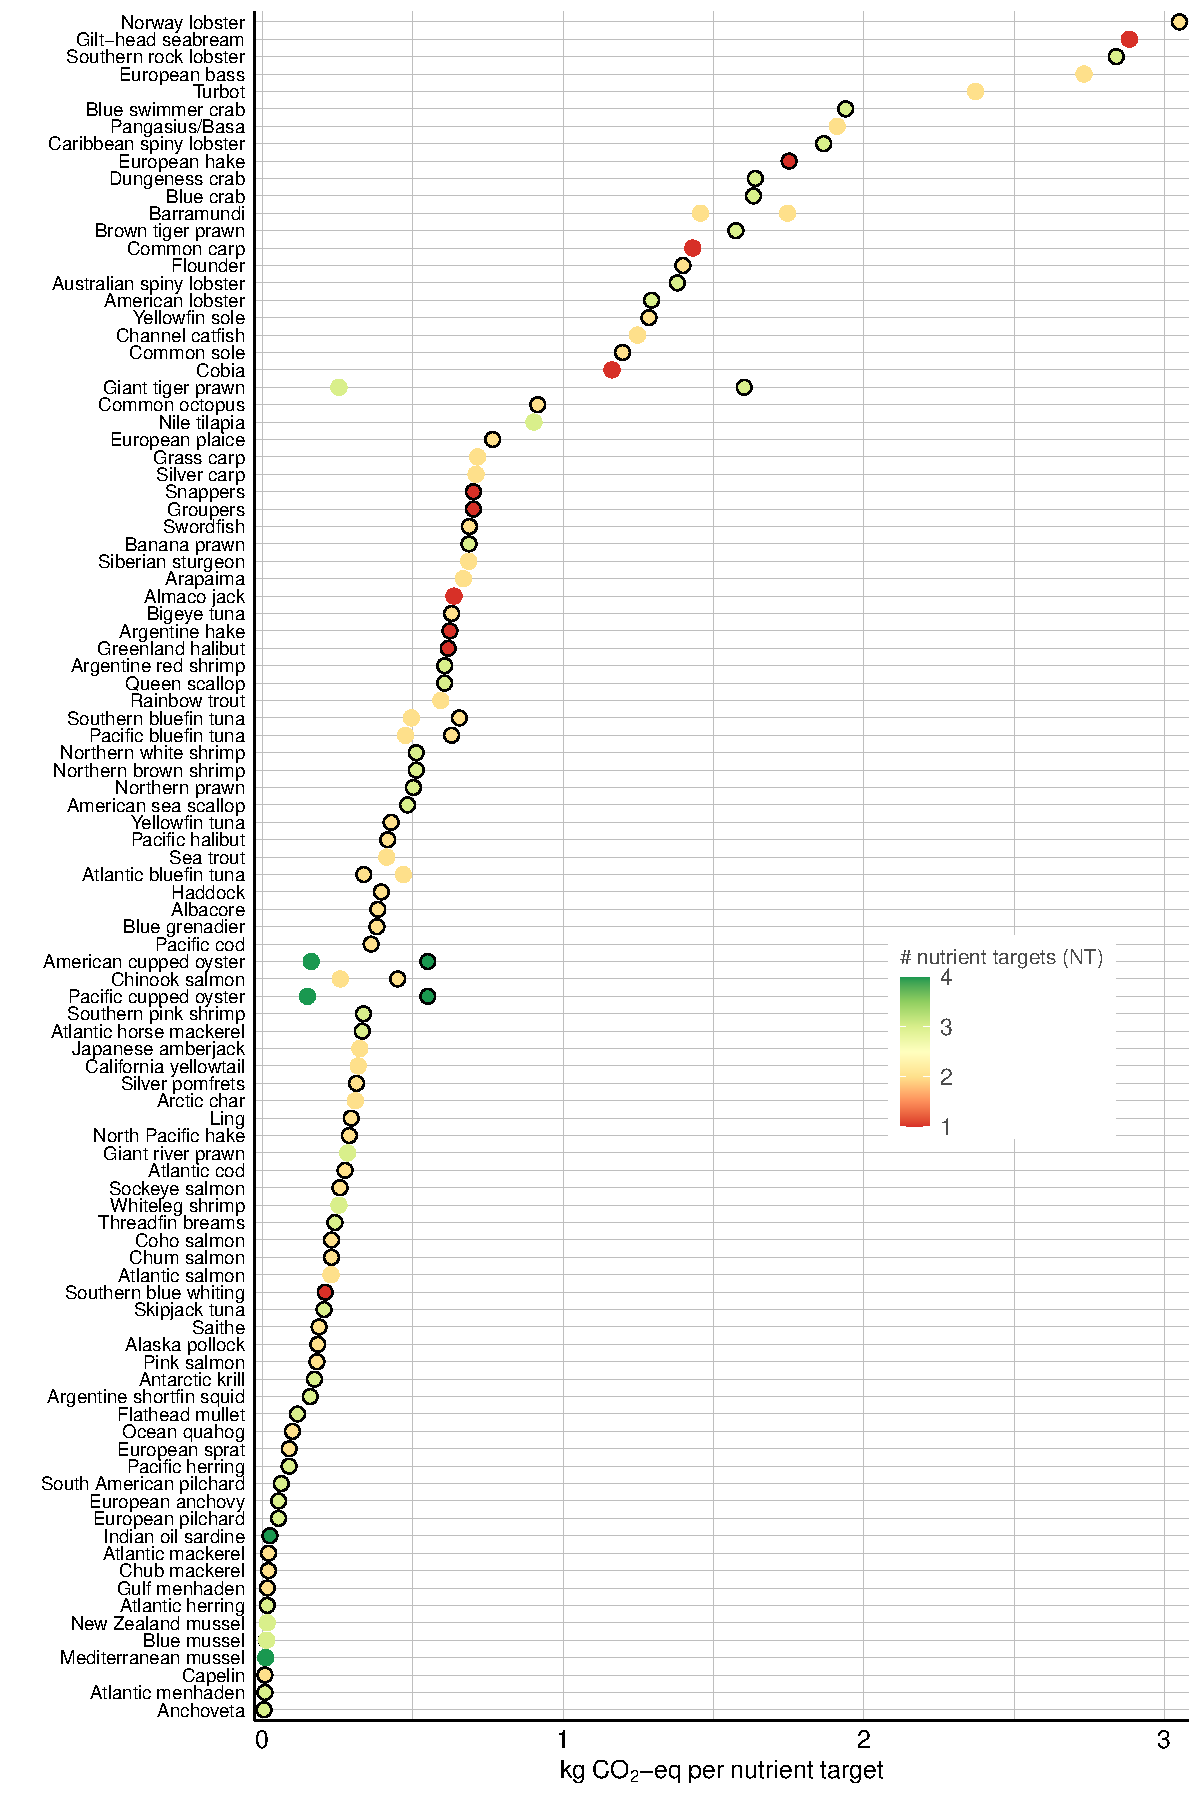
\includegraphics[height=0.8\textheight]{fig/final/FigureS3} \end{center}

\textbf{Fig. S3. Carbon emissions per nutrient target for all seafood
products in the carbon emissions database} Points are the mean kg CO2-eq
per nutrient target for each seafood species, where a nutrient target
was the recommended intake (adults 18-65 years old) contained in a 100 g
edible portion for 7 nutrients (calcium, iron, selenium, zinc, omega-3
fatty acids, vitamin A). Points are coloured by the number of nutrient
targets in a 100 g edible portion. Animal-source foods (beef, chicken,
lamb, pork) are included for comparison using CO2 values from (Clune et
al., 2017) and nutrient values from (Widdowson, n.d.).

\newpage

\begin{center}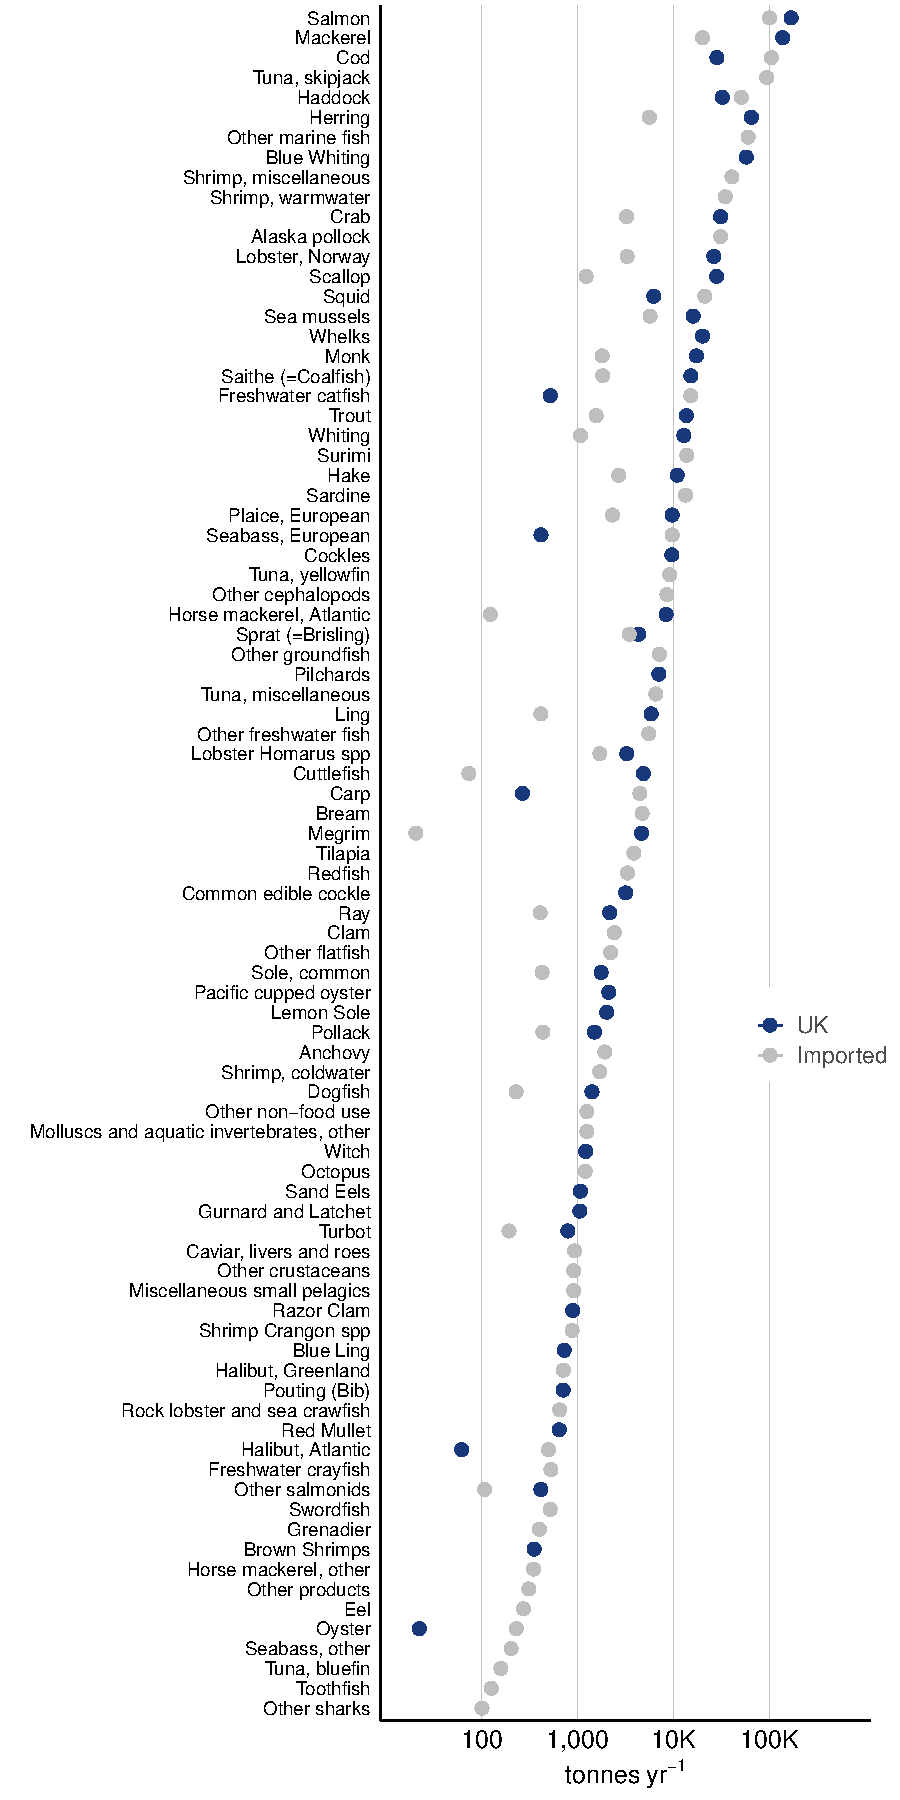
\includegraphics[height=0.8\textheight]{fig/final/FigureS2_UK_seafood} \end{center}

\textbf{Fig. S4. Seafood available for UK consumers.} Points are the
estimated UK production (blue, landings and farms) and imported (grey)
seafood per year, for all seafood with more than 100 tonnes total
production.

\newpage

\begin{center}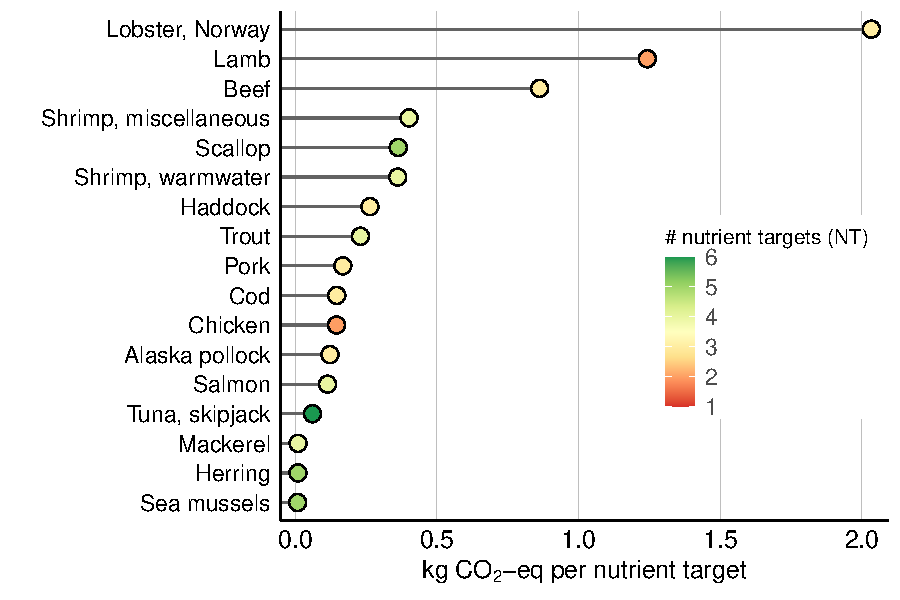
\includegraphics[height=0.8\textheight]{fig/final/Figure3} \end{center}

\textbf{Figure S5. Carbon emissions per nutrient target for UK seafood
products, for nine essential dietary nutrients.} Points are kg CO2-eq
per nutrient target (averaged across species), coloured by the number of
nutrient targets in a 100g portion. Targets were recommended intakes for
adults (18-65 years old) of nine nutrients (calcium, iron, selenium,
zinc, omega-3 fatty acids, vitamins A, D, B12, folate). Animal-source
foods (beef, chicken, lamb, pork) are included for comparison using CO2
values from (Clune et al., 2017) and nutrient values from (Widdowson,
n.d.).

\newpage

\begin{center}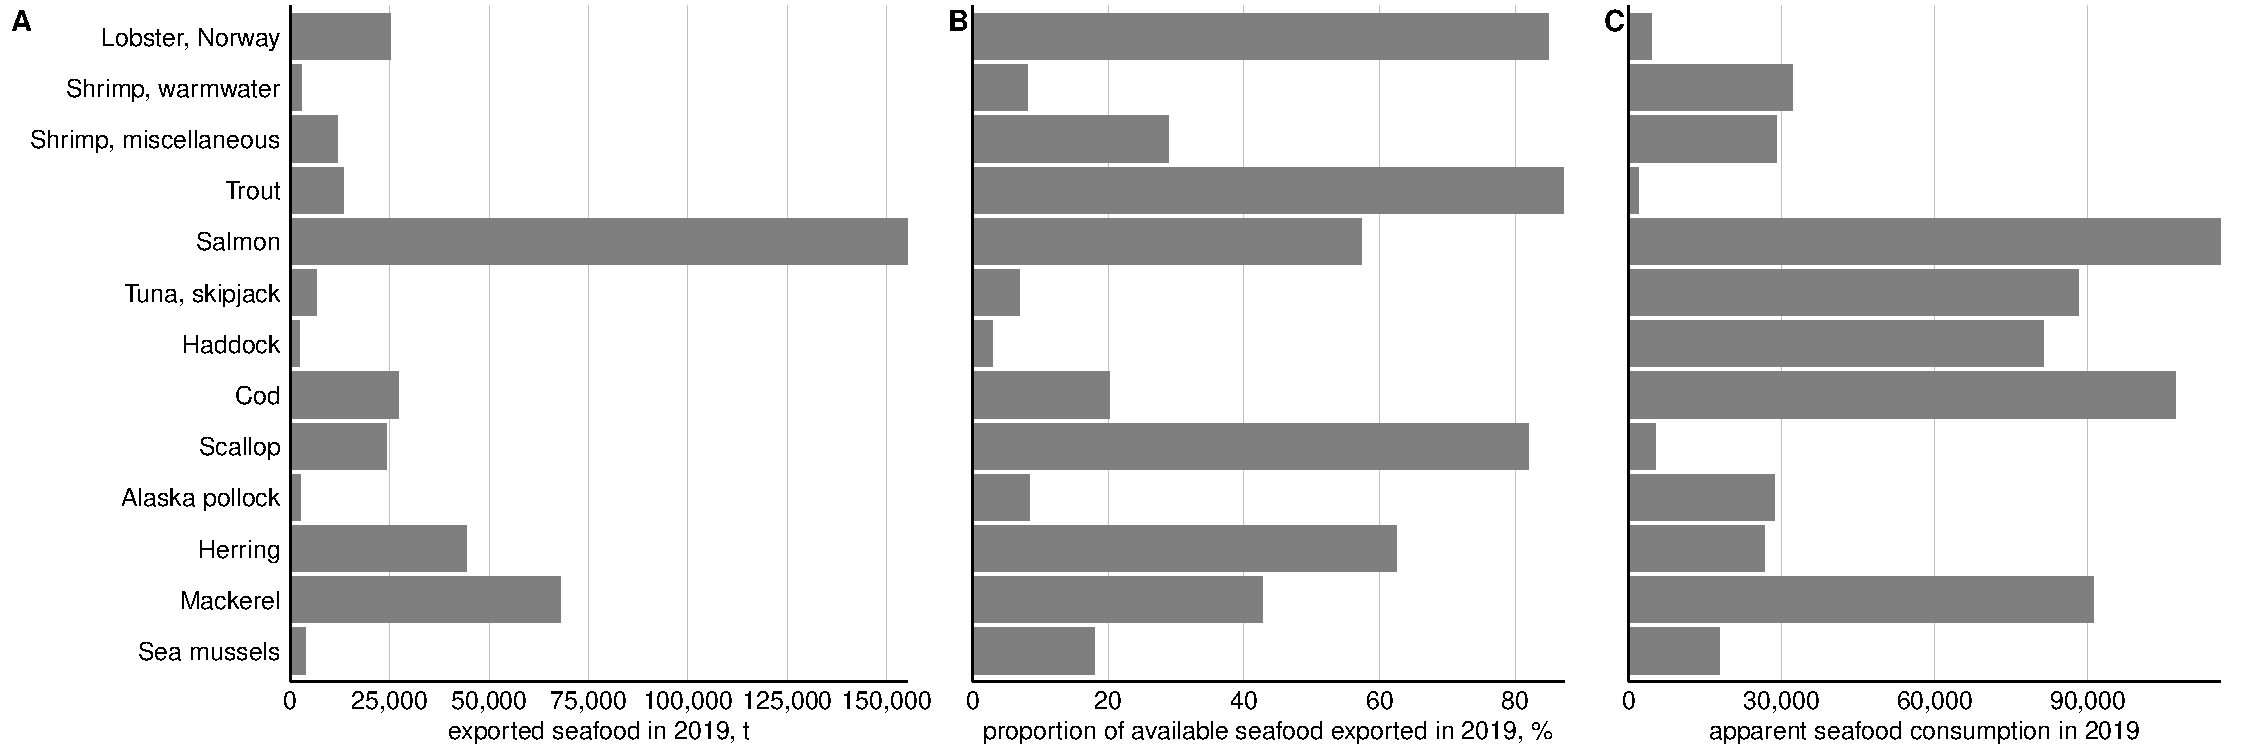
\includegraphics[height=0.8\textheight]{fig/final/FigureSX_UK_export} \end{center}

\textbf{Fig. S6. Seafood exported from the UK in 2019} A) Export volume
in tonnes of live weight, B) export volume as a proportion of available
seafood, and C) domestic use as a proportion of available seafood.
Seafood products shown had more than 100 tonnes total production
(i.e.~those in Fig. 2). Available seafood was the sum of landed, farmed,
imported and domestic use was the total available seafood minus exports,
using data for 2019.

\newpage

\begin{center}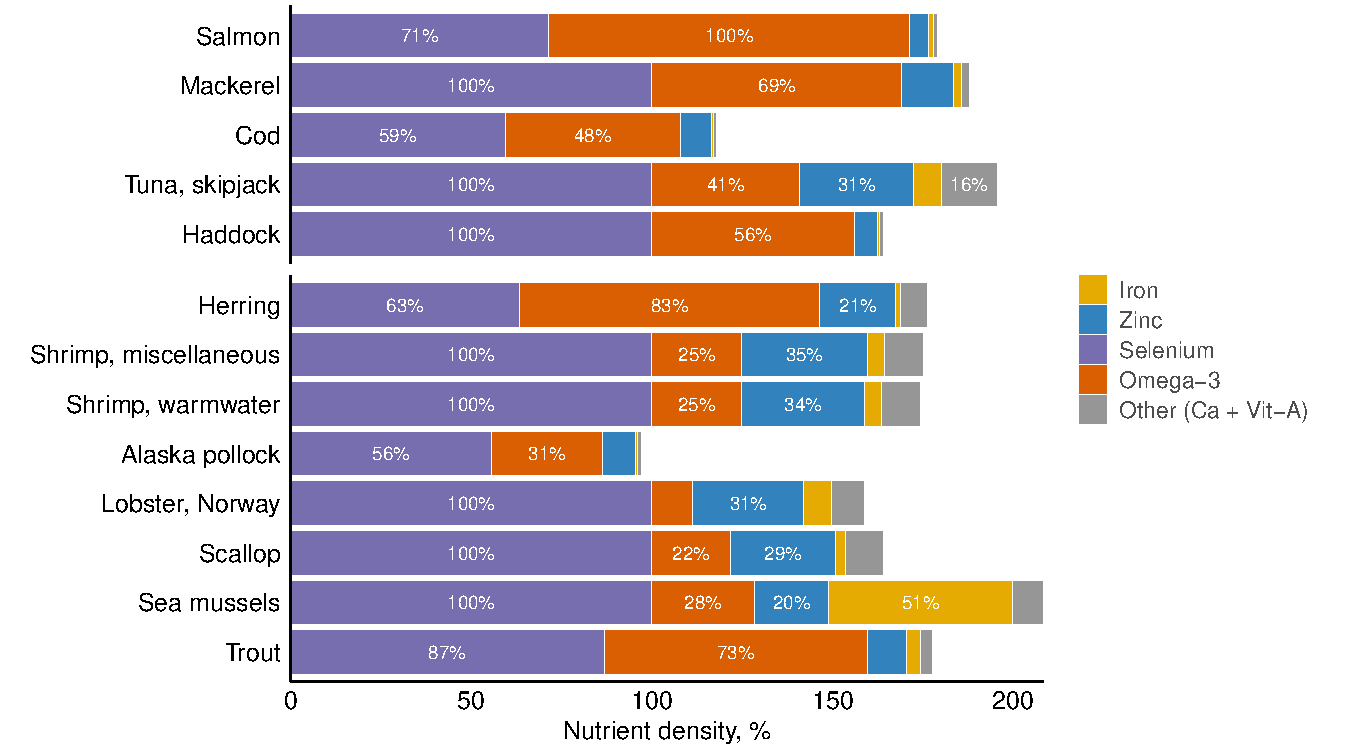
\includegraphics[height=0.8\textheight]{fig/final/FigureSX_UK_fournut_density} \end{center}

\textbf{Fig. S7. Nutrient density for major UK seafood products
estimated for five nutrients (calcium, iron, selenium, zinc, omega-3
fatty acids).} Nutrient density based on recommended daily intakes for
adults (18-65 years old), recalculated here for comparison with Fig. 1
(nutrient content of global seafood products).

\newpage

\begin{center}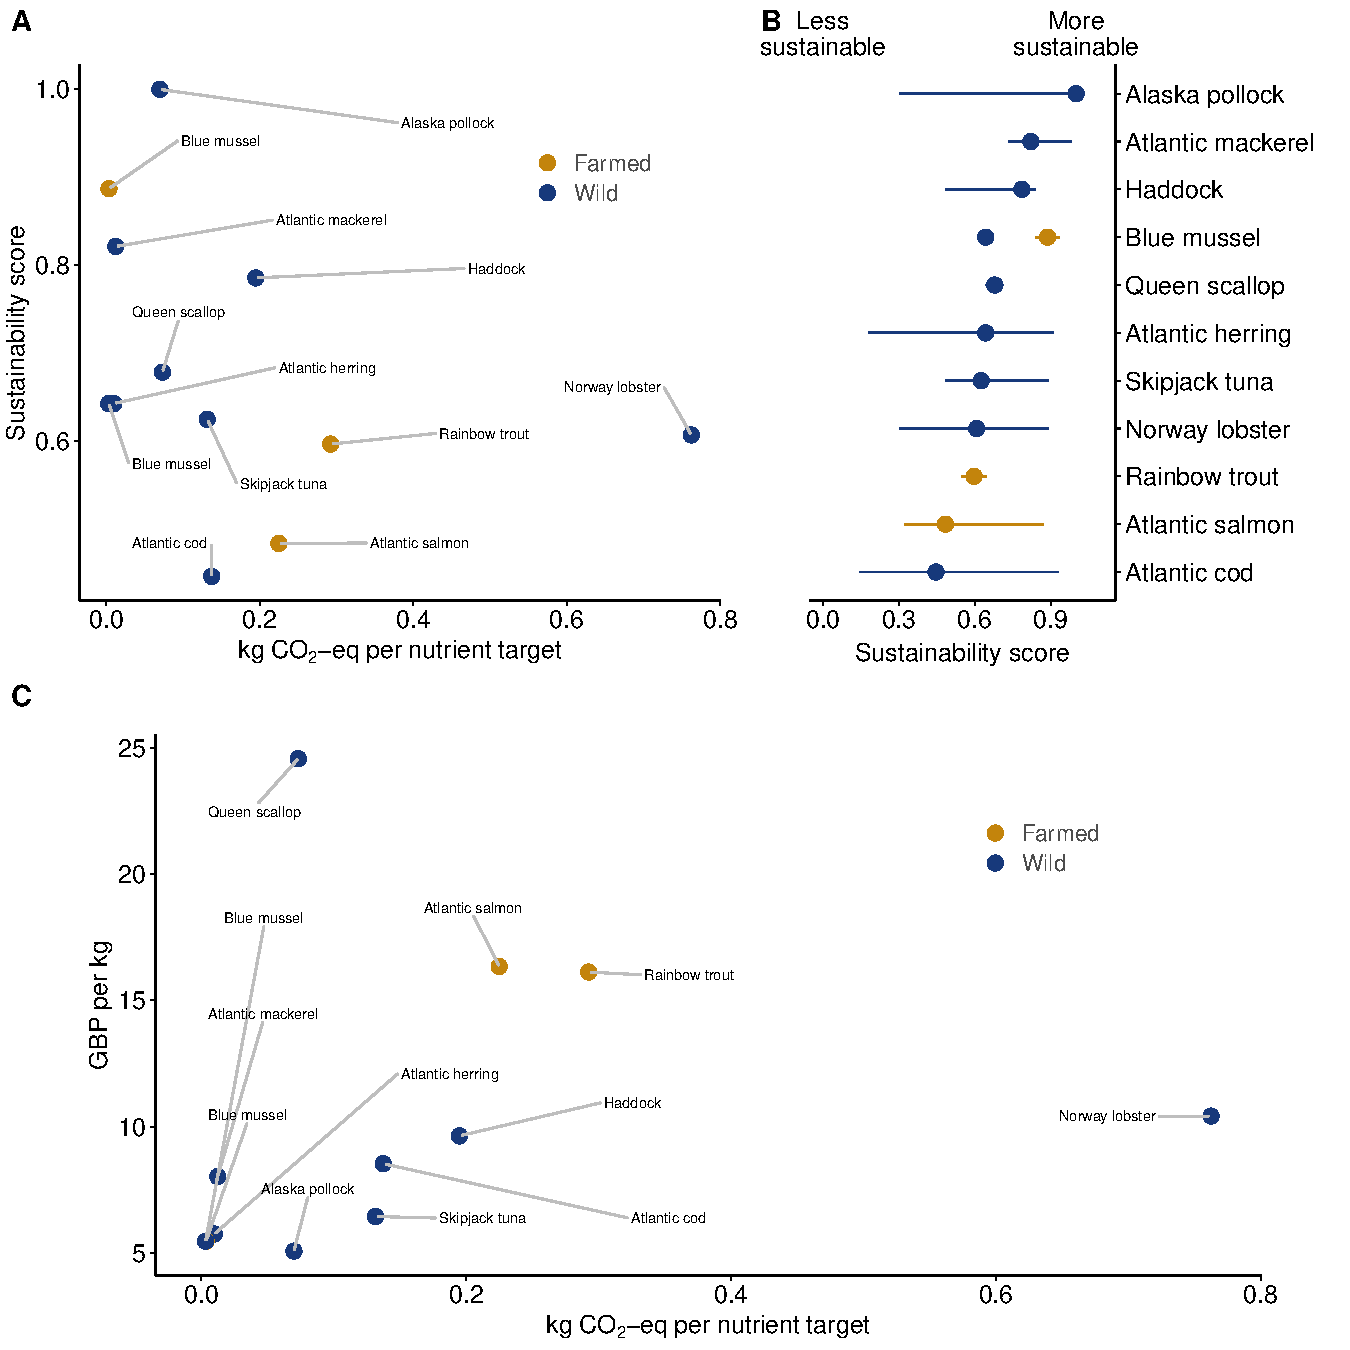
\includegraphics[height=0.8\textheight]{fig/final/FigureSX_GFGscore} \end{center}

\textbf{Fig. S8. Sustainability and price of UK seafood products.} A)
Carbon emissions per nutrient target by sustainability score, where
points are the mean sustainability score of each product against the
mean kg CO2-eq per nutrient target. B) is the range in sustainability
scores by seafood product and C) is the price per kg (Seafish 2021)
against kg CO2-eq per nutrient target. Sustainability scores were
rescaled such that 0 = low sustainability and 1 = high sustainability,
and kg CO2-eq per nutrient target was estimated from recommended intakes
of nine nutrients (calcium, iron, selenium, zinc, omega-3 fatty acids,
vitamins A, B12, D and folate).

\newpage

\begin{center}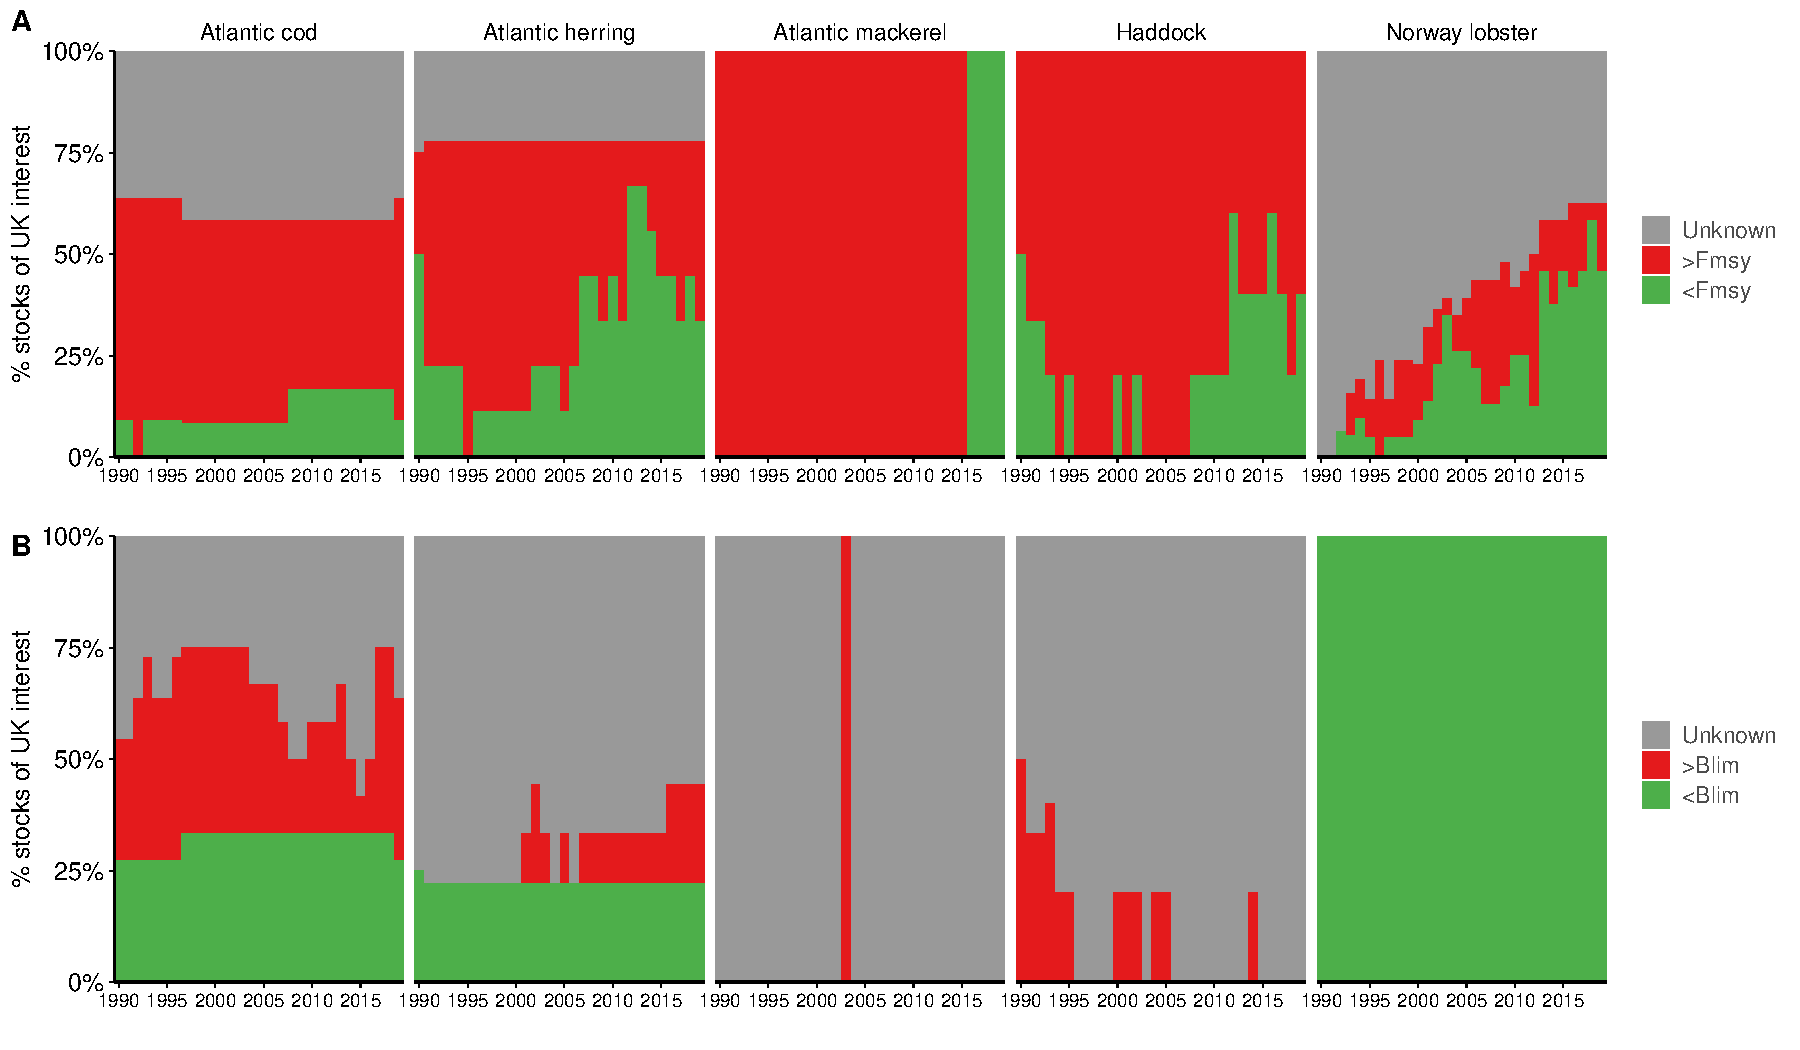
\includegraphics[height=0.8\textheight]{fig/final/FigureSX_stock_status} \end{center}

\textbf{Fig. S9. Pressure and state thresholds for wild fisheries stocks
relevant to UK seafood production from 1990-2019.} Bars indicate the
proportion of stocks that are underfished (green), overfished (red), or
data deficient (unknown), according to estimates of fishing mortality
(A, F\_MSY\_) or spawning stock biomass (B\_lim\_). Data from CEFAS
(Lynam et al.~2021)..

\end{document}
